\chapter{理论模型}
\section{利用词嵌入技术构造新型元数据}
\subsection{文件名、目录名的向量化}
在Unix文件系统中,任意文件或目录在被创建时,均会被分配一个唯一的ID,也就是Inode序号,以此作为唯一的标识以便于后续各种文件操作。Inode序号只与文件创建先后相关,是一种one-hot的表示方式。那么能否效仿自然语言处理中词嵌入的思想,建立一种能够包含文件或目录之间关联性的表征方式?

文件系统层次结构规范(Filesystem Hierarchy Standard,FHS)\cite{fhs}是由Linux基金会在1994年发起,旨在规范Linux各发行版和其他类Unix系统下文件目录结构的业界统一标准,至今已发展演变到FHS-3.0(2015年)。在FHS定义的目录结构规范下,Linux操作系统的目录组织结构和命名受到了明确严格的约束,例如:

{\color{red}这里做成表格!}
\begin{itemize}
    \item /:根目录。
    \item /bin:系统执行文件目录。
    \item /boot:启动文件目录。
    \item /dev:驱动设备目录。
    \item /etc:系统配置文件目录。
    \item /lib, /usr/lib, /usr/local/lib:系统使用的函数库目录。
    \item ......
\end{itemize}

如果将一个文件的完整路径(如/usr/lib/python2.7/)视为一个句子,各级目录视为单词,我们假定类似于自然语言中的分布式假设同样成立,即:同一目录下的文件或目录具有类似的含义。直观上看,这个假设是合理的,例如/bin目录下的bash,rm,cp文件等均为可执行命令,/usr/lib/python2.7/目录下均为Python的库文件。在此假设成立的前提下,本节将介绍如何使用Skip-gram模型,对给定的Unix文件系统目录下所有文件名、目录名进行向量化。

\subsubsection*{语料库的生成}
众所周知,任何机器学习模型都离不开数据,自然语言处理领域的数据集通常被称为语料库(Corpus)。任何语言学的研究或者自然语言模型的建立都必须建立在大量的语料之上,否则无论是基于规则方法还是统计方法建立的模型都将失效。

为了建立文件路径相关的“语料库”,我们将从根目录(或文件系统的挂载点)开始,通过常规的遍历算法将此目录下所有文件、目录的完整路径逐行写入到一个文本文件,作为模型的训练数据集。语料库生成后,相应地可以得到一个词汇表$V$。
{\color{red}此处插入遍历算法}

\subsubsection*{利用Skip-gram模型训练文件和目录名的词向量}
给定总单词数量为$T$的语料库,其词汇表$\mathcal{V}$=\{\textit{bin,boot,dev,...}\},词汇数量为$W$。
%其中任意一个词可用其在词汇表中的序号表示:$w \in \{1,\dots,W\}$。
那么该语料库可表示为一个由$T$个词向量组成的序列:$\mathbf{w}_1, \mathbf{w}_2, \dots, \mathbf{w}_T$。Skip-gram模型的目标就是建立一个从词汇表到$d$维向量空间的映射$model:\mathcal{V} \rightarrow \mathbb{R}^d$,使以下对数极大似然函数达到最大:
\begin{equation}
    \label{eq:origin_object}
    \frac{1}{T}\sum_{t=1}^T \sum_{c \in \mathcal{C}_t} \log p(\mathbf{w}_c | \mathbf{w}_t),
\end{equation}
取负号得到损失函数:
\begin{equation}
    L(\theta)= -\frac{1}{T}\sum_{t=1}^T \sum_{c \in \mathcal{C}_t} \log p(\mathbf{w}_c | \mathbf{w}_t),
\end{equation}

其中,$\mathcal{C_t}$表示某中心词$\mathcal{w}_t$的上下文中出现过的词的集合。以路径\textit{/usr/local/lib/python}为例,若取上下文窗口大小为1,那么中心词$\mathcal{w}_t$=\textit{lib}的上下文集合$\mathcal{C_t}$=\{\textit{local,python}\},在文件系统的情境下,此处“上下文”隐含的语义是指\textit{usr},\textit{python}分别与\textit{lib}有着父子目录的关系。对于任意样本$(\mathbf{\mathcal{w}}_t,\mathbf{\mathcal{w}}_c)$,我们可用归一化函数softmax来定义单词$\mathcal{w}_c$在中心词$\mathbf{\mathcal{w}}_t$的上下文中出现的条件概率:
\begin{equation}
    \label{eq:softmax}
    p(\mathbf{w}_c | \mathbf{w}_t)=\frac{ e^{ \mathbf{w}_t^{\top} \mathbf{w}_c} }{ \sum_{j=1}^W e^{\mathbf{w}_t^{\top} \mathbf{w}_j}} 
\end{equation}

\begin{figure}[htp]
\centering
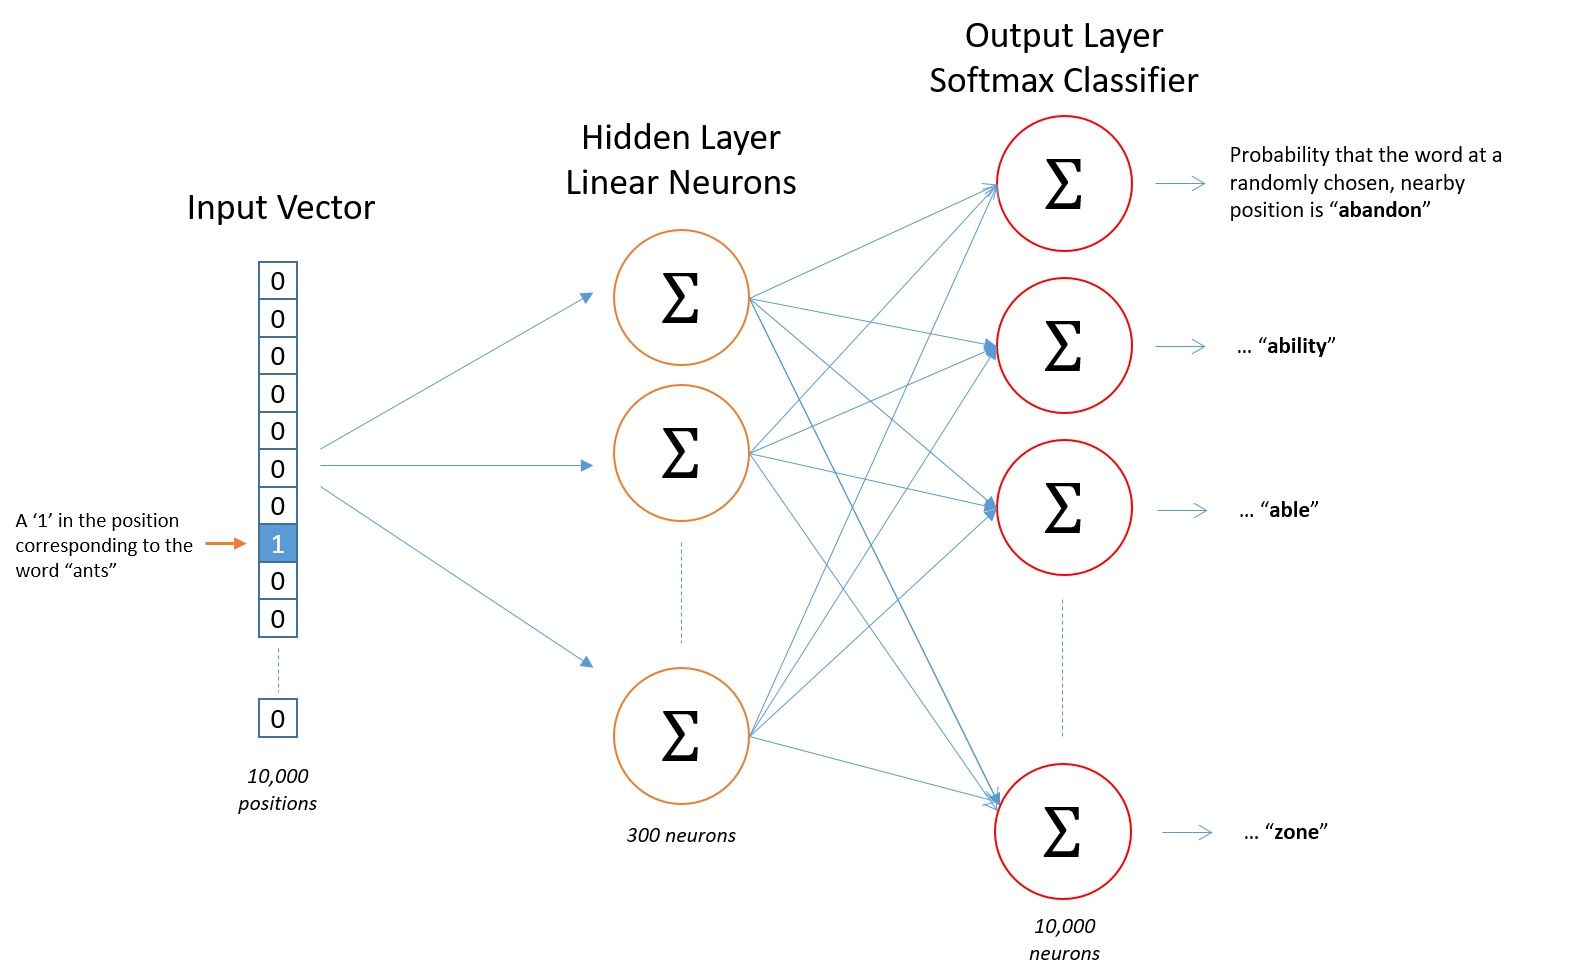
\includegraphics[width=\textwidth]{word2vec_nn}
\caption{Skip-gram模型网络}
\label{fig:word2vec_nn}
\end{figure}
如图\ref{fig:word2vec_nn},Skip-gram模型是一个三层神经网络,输入为词汇表中单词的初始向量,即$W$维的one-hot编码。隐层由$d$个神经元组成,没有激活函数,只有权值。训练收敛后隐层的$W\times d$的权值矩阵就是词汇表内所有词向量的集合。输出层为上文所述的softmax函数,最终结果是一个$W$维的向量,每个分量表示对应的单词与输入词存在上下文关系的概率。

当语料库规模较大,词汇表内单词较多时,采用softmax函数的计算复杂度过高。一种优化方式是使用层次化softmax(Hierarchical softmax)\cite{Hierarchical_softmax}。另一种计算复杂度更低,且同样能保证对原有softmax层拟合精度的优化方式是负采样(Negative sampling)。该方法将原来的预测上下文的问题转化为一系列独立的二分类问题,即,在选定中心词后,对词汇表中其他单词依次判定是否在中心词附近出现。


对任意中心词$\mathbf{w}_t$,用交叉熵损失函数(Cross-entropy Loss)代替原来的损失函数
\begin{equation}
    \label{eq:loss_of_t}
    L_t(\theta) = -\left( 
        \sum_{c \in \mathcal{C}_t} \log(p(\mathbf{w}_c | \mathbf{w}_t))+\sum_{c \in \mathcal{N}_t} \log(1-p(\mathbf{w}_c | \mathbf{w}_t)) 
    \right)
\end{equation}
其中$\mathcal{C}_t$表示中心词$w_t$的上下文单词集合(正样本),$\mathcal{N}_t$表示词汇表中,与$w_t$不存在上下文关系的单词(负样本)中随机抽取的若干噪声词。

由于任意单词与中心词是否上下文被视为独立事件,可用sigmoid函数拟合条件概率
\begin{equation}
    p(\mathbf{w}_c | \mathbf{w}_t) = \frac{1}{1+e^{-\mathbf{w}_t^{\top} \mathbf{w}_c}} = \sigma(\mathbf{w}_t^{\top} \mathbf{w}_c)
\end{equation}

代入\ref{eq:loss_of_t}并按$t$累加求平均,得到最终的损失函数:
\begin{equation}
    L(\theta) = \frac{1}{T}\sum_{t=1}^{T} \left[
        \sum_{c \in \mathcal{C}_t} \log(\sigma(\mathbf{w}_t^{\top} \mathbf{w}_c)) + \sum_{c \in \mathcal{N}_t} \log(\sigma(-\mathbf{w}_t^{\top} \mathbf{w}_c))
    \right]
\end{equation}


%\begin{equation}
%    \label{eq:neg}
%    \log(1+e^{-\mathbf{w}_t^{\top} \mathbf{w}_c})+ \sum_{n \in \mathcal{N}_{t,c} }\log(1+ e^{\mathbf{w}_t^{\top} \mathbf{w}_n})
%\end{equation}
%
%
%用sigmoid函数$\sigma(x) = \log(1+e^{-x})$与公式\ref{eq:neg}代入目标函数\ref{eq:origin_object}得到最终的目标函数:
%\begin{equation}
%    \frac{1}{T} \sum_{t=1}^{T} \left[ \sum_{c \in \mathcal{C}_t} \sigma(\mathbf{w}_t^{\top} \mathbf{w}_c) + \sum_{n \in \mathcal{N}_{t,c}} \sigma(-\mathbf{w}_t^{\top} \mathbf{w}_n) \right]
%\end{equation}

经过以上优化后,Skip-gram模型训练的计算复杂度大大缩小。隐层的$W\times d$的权值矩阵$\theta$通过常规的随机梯度下降训练收敛后,作为最终词汇表$\mathcal{V}$的词向量模型。

\subsection{引入子词模型}
%阐述文件系统内命名与人类自然语言的区别,与前文FastText中的子词模型呼应
\subsection{路径向量}
%注意区分绝对路径、工作路径、挂载点等造成的差异
\section{基于门控神经网络的热点数据识别}
\subsection{问题描述}
%设文件系统进行文件向量化处理后,所有文件向量($d$维)组成的集合记为$\mathcal{F} \subset \mathbb{R}^d$。在某工作负载的生命周期内对其文件访问进行追踪,将追踪日志转化为$d$维路径向量序列$\mathcal{S}=\{\mathbf{x}_1, \mathbf{x}_2,\dots, \mathbf{x}_T\}$。
%设上下文窗口大小为$N$,即
%在任意时刻$t$,追踪模块对前$N$次访问构成的日志序列$\{\mathbf{x}_{t-N+1}, \dots, \mathbf{x}_t\}$记为$\mathcal{L_t}$。
%定义该时刻的上下文序列$\mathcal{C}_t = \{ \mathbf{x}_{t-N+1}, \dots, \mathbf{x}_{t+N} \}$为正类样本(热文件),其余所有文件$\mathcal{N}_t = \mathcal{F} - \mathcal{C}_t$为负样本(冷文件)。
%
%在以上定义下,热点数据识别可转化为如下二分类问题的求解,其目标是:建立模型$M$,以$\mathcal{L}_t$为输入,计算这段访问序列所隐含的访问模式$\mathbf{h}_t$($d$维向量)。同时定义函数$f:\mathbb{R}^d \times \mathcal{F} \rightarrow [0,1]$,其含义为:访问模式$\mathbf{h}_t$下,文件$\mathbf{x}$是热点文件的概率。最后,为保证冷热文件的分类不会因为计算结果频繁扰动,设置合理的阈值$0<\alpha<\beta<1$来判定冷热。

设文件系统进行文件向量化处理后,所有文件向量($d$维)组成的集合记为$\mathcal{F} \subset \mathbb{R}^d$。在某工作负载的生命周期内对其文件访问进行追踪,将追踪日志转化为$d$维路径向量序列$\mathcal{S}=\{\mathbf{x}_1, \mathbf{x}_2,\dots, \mathbf{x}_T\}$。

在给定上述数据集的条件下,热点数据识别可转化为如下动态二分类问题求解:建立模型计算任意时刻$t$所隐含的访问模式$\mathbf{h}_t$。同时定义函数$f:\mathbb{R}^d \times \mathcal{F} \rightarrow [0,1]$,其含义为:访问模式$\mathbf{h}_t$下,文件$\mathbf{x}$是热点文件的概率。最后,为保证冷热文件的分类不会因为计算结果频繁扰动,设置合理的阈值$0<\alpha<\beta<1$来判定冷热。


\subsection{基于门控神经网络的模型设计}

在当前大数据背景下,海量小文件访问的读写性能是制约存储系统整体性能的瓶颈之一。在针对此类工作负载进行访问模式分析与热点数据识别时,上节所定义的问题规模将会十分巨大:应用生命周期内累积的访问序列过长,模型应具备长期记忆的功能。为此,本文采用门控神经网络单元作为访问模式的分析模型。

{\color{red}如图},

\subsubsection*{1.输入层设计}

设上下文窗口大小为$N$。在任意时刻$t$,我们将最近$N$次文件访问构成的日志序列$\{\mathbf{x}_{t-N+1}, \dots, \mathbf{x}_t\}$作为输入序列$\mathcal{L_t}$。

\subsubsection*{2.隐层设计}
如图所示,本文采用单层GRU来计算某一时刻隐含的文件访问模式$h_t$。前向传播的具体计算过程如下:

在时刻$t$, 我们用$h_t^{(j)}$来表示隐状态$\mathbf{h}_t$的第$j$个分量,由前一时刻隐状态$h_{t-1}^{(j)}$与候选隐状态$\tilde{h}_t^{(j)}$加权求和计算:
\begin{equation}
    h_t^{(j)} = (1-z_t^{(j)}) h_{t-1}^{(j)} + z_t^{(j)}\tilde{h}_t^{(j)},
\end{equation}
其中$z_t$为更新门(update gate),由当前时刻输入$\mathbf{x_t}$和上一刻的隐状态$\mathbf{h_{t-1}}$计算获得:
\begin{equation}
z_t^{(j)} = \sigma(W_z \mathbf{x}_t + U_z \mathbf{h}_{t-1})^{(j)}
\end{equation}
候选隐状态$\tilde{h}_t^{(j)}$的计算如下:
\begin{equation}
    \tilde{h}_t^{(j)} = \tanh(W \mathbf{x}_t + U (\mathbf{r}_t \odot \mathbf{h}_{t-1}))^{(j)}
\end{equation}
此处$\mathbf{r}_t$是重置门(reset gate),运算符号$\odot$表示行列相同的矩阵之间的逐元素相乘(Hadamard product)。此处表示$\mathbf{r}_t$的第$j$个元素与隐状态$h_{t-1}$的第$j$个元素相乘。

重置门$r_t$由以下表达式求得:
\begin{equation}
    r_t^{(j)} = \sigma(W_r \mathbf{x}_t + \mathbf{U}_r \mathbf{h}_{t-1})^{(j)}
\end{equation}

\subsubsection*{3.输出层设计}

如上文所述,我们构造了单层GRU来计算隐状态$h_t$,为了赋予$h_t$识别热点文件的功能,我们构造函数$f:\mathbb{R}^d \times \mathcal{F} \rightarrow [0,1]$用于计算在状态$\mathbf{h}_t$下,文件$\mathbf{x}_t$是热数据的条件概率:
\begin{align}
    \begin{split}
    p(\mathbf{x} | \mathbf{h}_t) &= f(\mathbf{h}_t,\mathbf{x}) \\
                                &= \sigma(\mathbf{h}_t^{\top} \mathbf{x}) \\
                                &= \frac{1}{1+e^{-\mathbf{h}_t^{\top} \mathbf{x}}}
    \end{split}
\end{align}

与常规的文本分类任务不同,文件访问序列组成的样本不带标签,或者说冷、热标签是随着时刻$t$动态改变的。在实际应用场景下,$t$时刻前访问尚未结束的文件,以及接下来即将访问的文件都是热数据,然而缓存容量是有限的,可以被纳入热数据的总量应与缓存容量呈正相关。为简化模型起见,此处设定与时间无关,只与缓存容量相关的超参数$M$,将文件序列$\{ x_{t-M+1},\dots,x_t,\dots,x_{t+M} \}$共计$2*M$条文件标记为正类样本集$C_t$,其余文件为冷数据。

通常冷文件数量近似于文件总数$|\mathcal{F}|$,考虑到实际文件系统中总文件数量巨大,将所有冷文件纳入负类样本将带来巨大的计算量。为此,本文借鉴Skip-gram算法中采用的负采样(Negtive sampling)的思想,对冷文件集随机采集$K$个样本组成负类样本集$\mathcal{N}_t$。

为训练该模型,采用二分类最常用的交叉熵损失函数:
\begin{equation}
    L(\theta) = \frac{1}{T-2M}\sum_{t=M}^{T-M+1} \left[
        \sum_{x \in \mathcal{C}_t} \log(p(x_i | h_t)) + 
        \sum_{x \in \mathcal{N}_t} \log(-p(x_i | h_t))
    \right]
\end{equation}

其中,待训练的参数$\theta$为GRU中各个部件的权重矩阵$W_z, U_z, W, U, W_r, U_r$,训练采用时序后向传播算法(Backpropagation Through Time)。要设置和调优的超参数包括输入序列长度$N$,与缓存容量正相关的热文件样本数$M$,以及负样本采样数$K$。

%指标以命中率、错判率为主,即准确率召回率?
\section{本章小结}